Neste apêndice, mostram-se os principais resultados da análise descritiva de dados. 
Começa-se mostrando os gráficos de barra dos atributos eliminados devido a
\textit{missing values}. Em seguida, as tabelas mostrando a diferença na capacidade
de formar, de acordo com o curso e com a idade são apresentadas. Seguindo isso,
mostram-se a mudança nos valores de alguns atributos. Por fim, apresentam-se os
gráficos de barra e histogramas para os atributos. 

\section{Atributos Eliminados devido a Missing Values} \label{graf_miss_value}
\par Eliminaram-se os atributos raça e tipo da escola, pela quantidade de
\textit{missing values}
ser superior a 40\%.  A Figura \ref{atr_race} mostra o gráfico de barra para o
atributo raça, enquanto que a Figura \ref{atr_school_type} mostra o gráfico de barra
para o atributo tipo da escola.  
    % raça
    \begin{figure}[!ht]
        \centering
        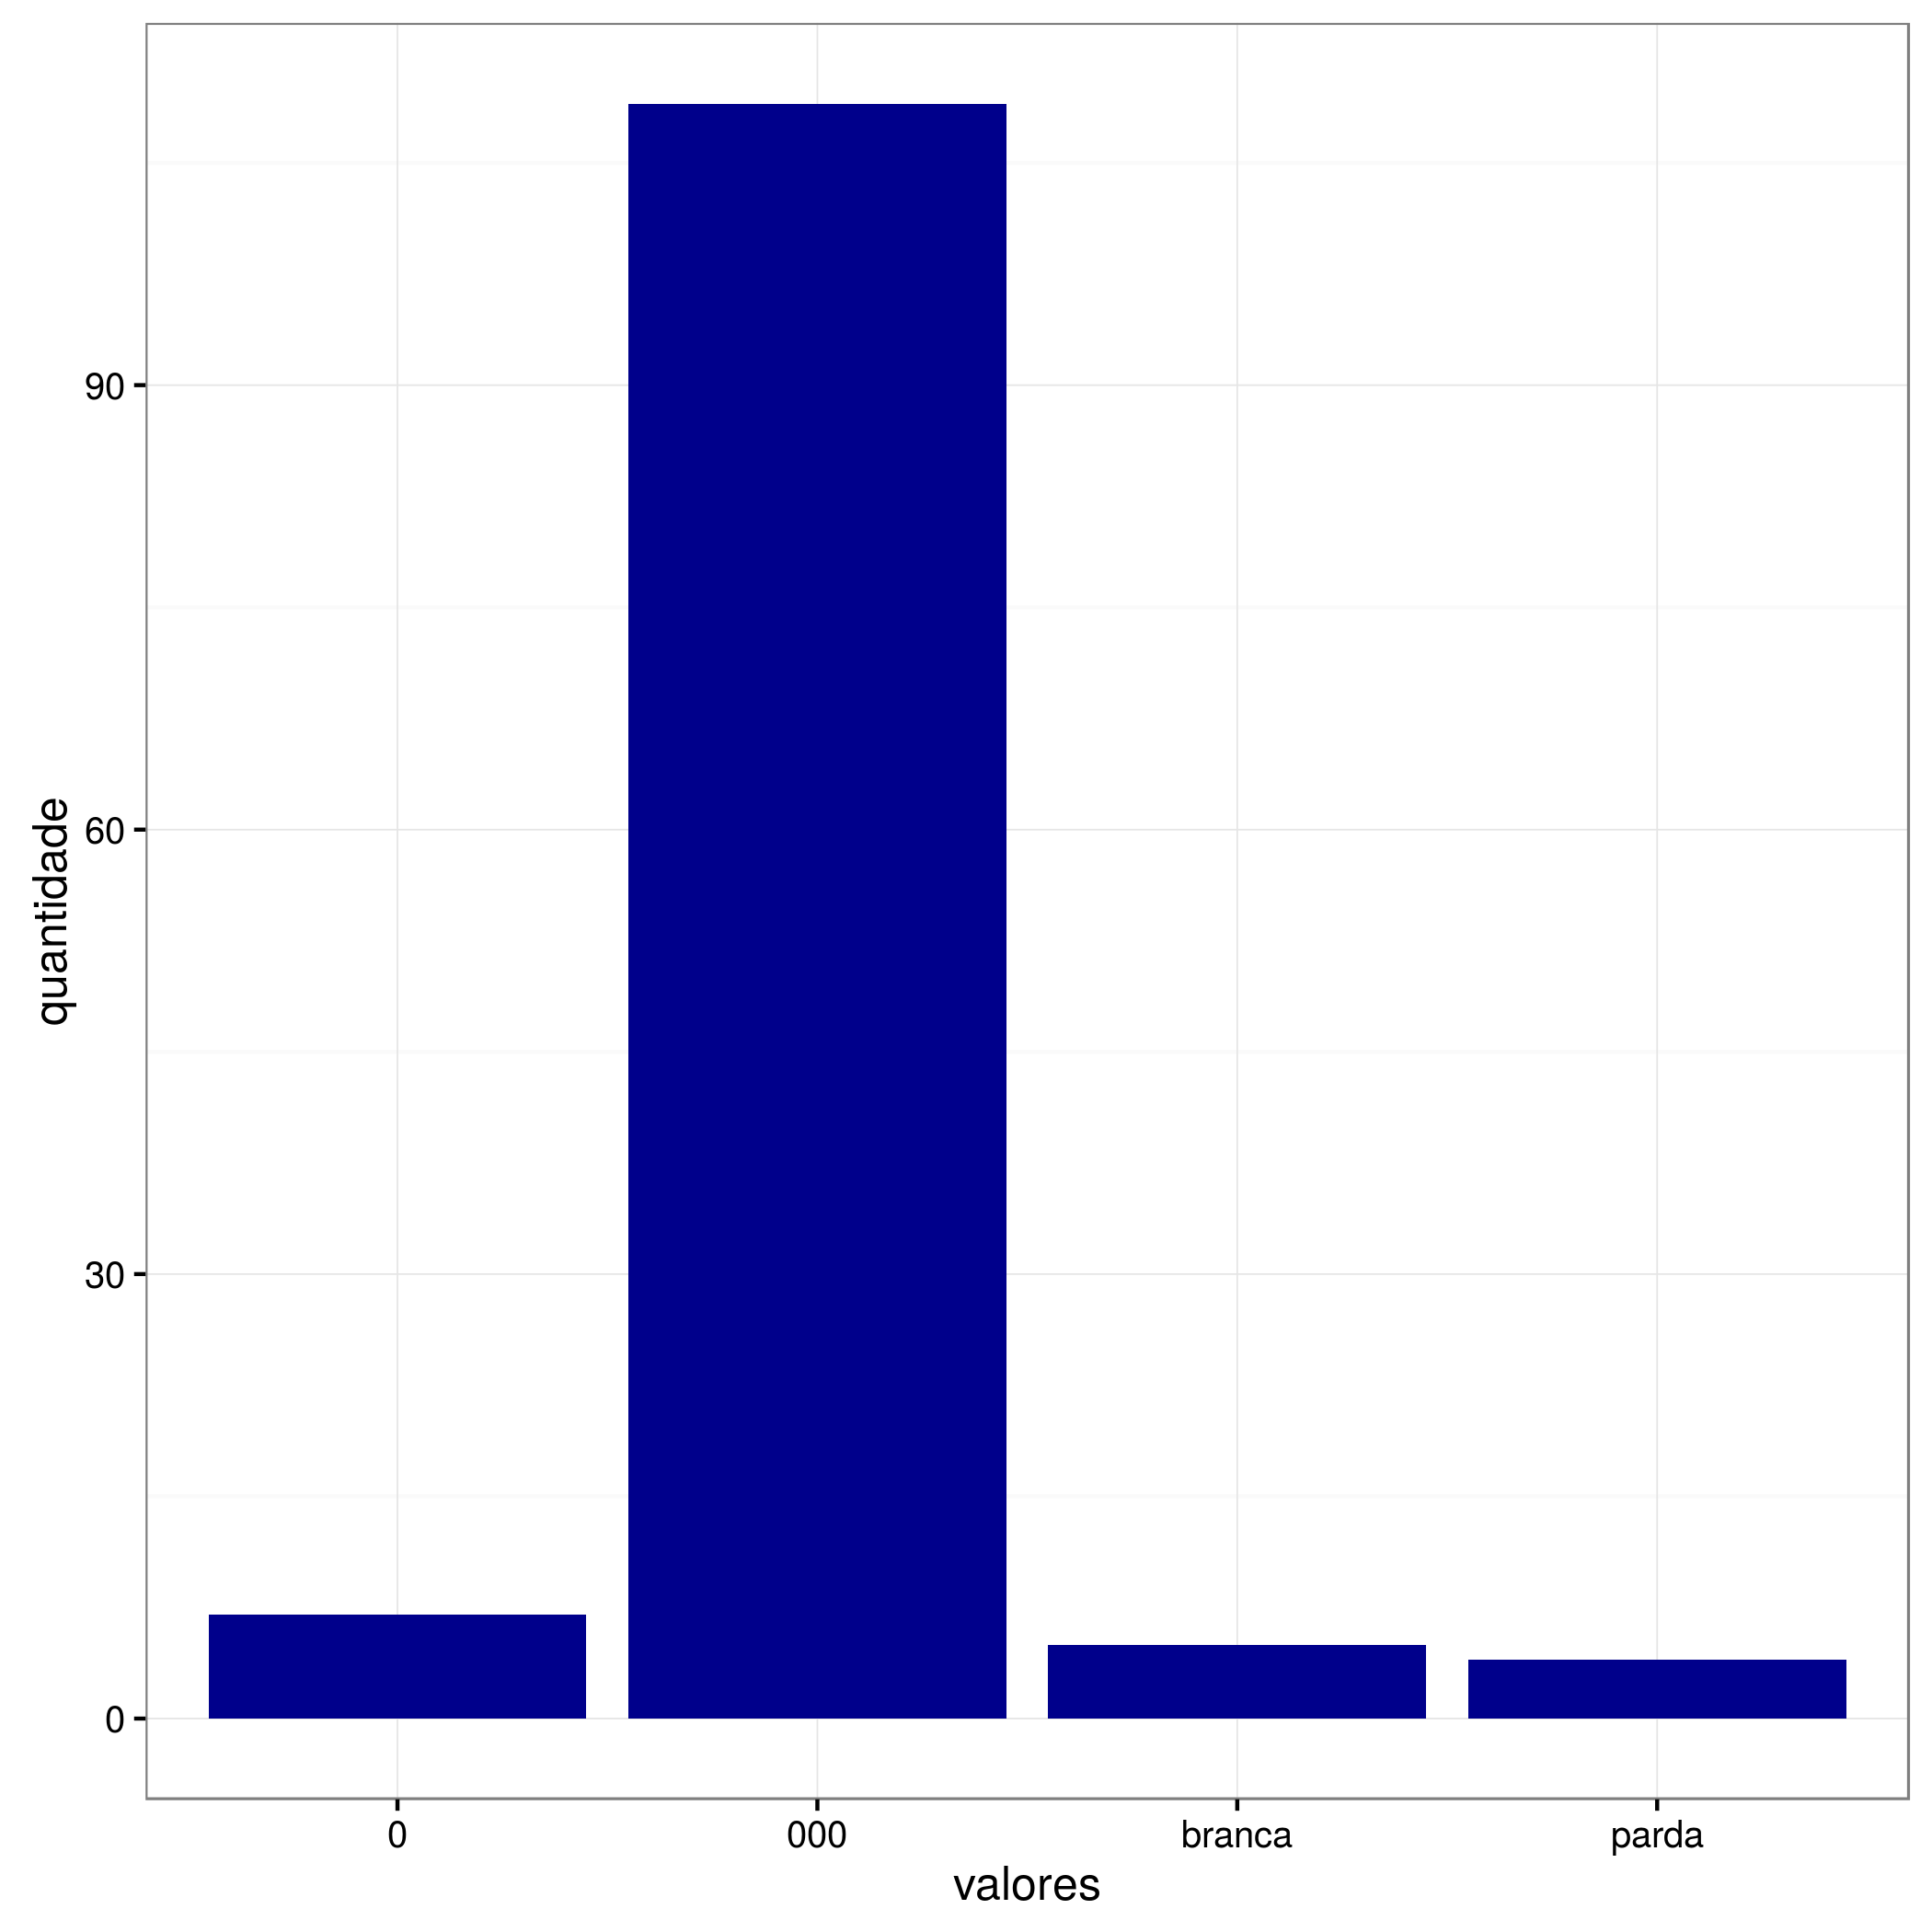
\includegraphics[width = 10cm]{all_students/race.png}
        \caption{Gráfico de Barra para Atributo Raça}
        \label{atr_race}
    \end{figure}

    % tipo da escola
    \begin{figure}[!ht]
        \centering
        \includegraphics[width = 10cm]{all_students/school_type.png}
        \caption{Gráfico de Barra para Atributo Tipo da Escola}
        \label{atr_school_type}
    \end{figure}

Conforme já dito, em ambos os casos, observam-se uma grande quantidade de valores
faltantes, de modo que tais atributos foram retirados de análises posteriores. 

\section{Impacto do Curso e Idade na Separação de Variáveis} \label{justificativa_4_base_dados}
Na análise preliminar por meio de estatística descritiva, analisou-se como a
distribuição dos atributos era afetada pelo curso do aluno, tendo-se constatado que a
influência do fator curso era bastante significativa. Isso pode ser visto na Tabela
\ref{justificativa_4_curso}.

\begin{table}
\caption{Percentagem de Alunos Capazes de Formar por Curso}
\begin{center}
\begin{tabular}[c]{| c | c |}
    \hline
    \textbf{Curso} & \textbf{Percentagem capaz de Formar} \\
    \hline
    Ciência da Computação (Bacharelado) & 42\% \\
    \hline
    Computação (Licenciatura) & 27\% \\
    \hline
    Engenharia da Computação & 20\% \\
    \hline
    Engenharia de Redes & 48\% \\
    \hline
    Engenharia de Software & 49\% \\
    \hline
    Engenharia Mecatrônica & 47\% \\
    \hline
\end{tabular}
\end{center}
\label{justificativa_4_curso}
\end{table}

\par Além do curso, a análise descritiva mostrou que a taxa de alunos que conseguem
formar é consideravelmente menor para estudantes mais velhos. Isso pode ser visto na
Tabela \ref{justificativa_4_idade}.

\begin{table}
\caption{Percentagem de Alunos Capazes de Formar por Idade}
\begin{center}
\begin{tabular}[c]{| c | c |}
    \hline
    \textbf{Idade} & \textbf{Percentagem capaz de Formar} \\
    \hline
    Estudantes que entraram com até 30 anos & 41\% \\
    \hline
    Estudantes que entraram com mais de 30 anos & 11\% \\
    \hline
\end{tabular}
\end{center}
\label{justificativa_4_idade}
\end{table}

\section{Mudança de Valores de Atributos} \label{just_mud_atr}
Conforme mencionado, os atributos forma de entrada e forma de saída tiveram seus
valores menos comuns agrupados em certas categorias. O gráfico de barra para o
atributo forma de ingresso, com seus valores originais, é mostrado na Figura
\ref{atr_way_in_org}. 
Por questões de legibilidade, a legenda no gráfico foi encurtada. Seu significado é
apresentado a seguir: 

    \begin{itemize}
    \item \texttt{vest}: Ingresso via Vestibular
    \item \texttt{ci}: Ingresso via Convênio-Int
    \item \texttt{to}: Ingresso via Transferência Obrigatória
    \item \texttt{ac}: Ingresso via Acordo Cultural PEC
    \item \texttt{ca}: Ingresso via Convênio Andifes
    \item \texttt{mc}: Ingresso via Matrícula Cortesia
    \item \texttt{tf}: Ingresso via Transferência Facultativa
    \item \texttt{ppp}: Ingresso via PEC-G Peppfol
    \item \texttt{pdcs}: Ingresso pois é portador de diploma de curso superior
    \item \texttt{vmc}: Ingresso via Vestibular para Mesmo Curso
    \end{itemize}

    \begin{figure}[!ht]
    \centering
    \includegraphics[width = 10cm]{all_students/way_in.png}
    \caption{Gráfico de Barra de Todos os Alunos, para o Atributo Forma de Ingresso}
    \label{atr_way_in_org}
    \end{figure}

O gráfico de barra para o atributo forma de saída, com seus valores originais, é
mostrado na Figura \ref{atr_way_out_org}. 
Por questões de legibilidade, a legenda no gráfico foi encurtada. Seu significado é
apresentado a seguir: 

    \begin{itemize}
    \item \texttt{dec}: Ex-Aluno pelo Decreto 477
    \item \texttt{deslg}: Saída por desligamento
    \item \texttt{form}: Saída pois conseguiu formar
    \item \texttt{null}: Saída por anulação de registro
    \item \texttt{trnsf}: Saída devido à Transferência
    \item \texttt{vest}: Saída devido à novo vestibular
    \end{itemize}

    \begin{figure}[!ht]
    \centering
    \includegraphics[width = 10cm]{all_students/way_out.png}
    \caption{Gráfico de Barra para Atributo Forma de Saída}
    \label{atr_way_out_org}
    \end{figure}


\section{Gráficos de Barra e Histogramas Para Atributos} \label{graf_bar_hist}
Mostra-se a seguir a distribuição dos atributos por meio de gráficos de barra e
histogramas. Essa parte de estatística descritiva levou em consideração a divisão dos
dados nas 4 bases de dados. Para se ter uma ideia de como uma determinada base de
dados se comportou em relação ao conjunto de todos os dados, fez-se também gráficos
de barra e histogramas considerando todos os alunos das 4 bases de dados.  

% todo: por alunos seniors
% atribute list to check 
    % 1. age 
    % 2. course
    % 3. grades?
    % 4. race?
    % 5. sex
    % 6. quota
    % 7. school type 
    % 8. way in 
    % 9. way out

    % 10. credit rate acc
    % 11. in condition
    % 12. drop rate
    % 13. fail rate
    % 14. hard rate 
    % 15. improvement rate
    % 16. ira
    % 17. pass rate
    % 18. position

% 1. age
\clearpage
\begin{figure}[!ht]
    \centering
    % figura 1
    \begin{subfigure}[b]{0.48\textwidth}
        \centering
        \includegraphics[width = 8cm, height = 7cm]{yng_ti/age.png}
        \caption{Alunos Jovens da FT}
    \end{subfigure}
    ~
    % figura 2
    \begin{subfigure}[b]{0.48\textwidth}
        \centering
        \includegraphics[width = 8cm, height=7cm]{yng_lic/age.png}
        \caption{Alunos Jovens da Licenciatura}
    \end{subfigure}

    % figura 3
    \begin{subfigure}[b]{0.48\textwidth}
        \centering
        \includegraphics[width = 8cm, height=7cm]{yng_comp/age.png}
        \caption{Alunos Jovens da Computação}
    \end{subfigure}
    ~
    % figura 4
    \begin{subfigure}[b]{0.48\textwidth}
        \centering
        \includegraphics[width = 8cm, height=7cm]{old_stu/age.png}
        \caption{Alunos Seniors}
    \end{subfigure}

    % figura 5
    \begin{subfigure}[b]{0.48\textwidth}
        \centering
        \includegraphics[width = 8cm, height=7cm]{all_students/age.png}
        \caption{Todos os Alunos}
    \end{subfigure}
    \caption{Atributo Idade, conforme os diferentes modelos}
\end{figure}

% 2. course
\clearpage
\begin{figure}[!ht]
    \centering
    % figura 1
    \begin{subfigure}[b]{0.48\textwidth}
        \centering
        \includegraphics[width = 8cm, height = 7cm]{yng_ti/course.png}
        \caption{Alunos Jovens da FT}
    \end{subfigure}
    ~
    % figura 2
    \begin{subfigure}[b]{0.48\textwidth}
        \centering
        \includegraphics[width = 8cm, height=7cm]{yng_lic/course.png}
        \caption{Alunos Jovens da Licenciatura}
    \end{subfigure}

    % figura 3
    \begin{subfigure}[b]{0.48\textwidth}
        \centering
        \includegraphics[width = 8cm, height=7cm]{yng_comp/course.png}
        \caption{Alunos Jovens da Computação}
    \end{subfigure}
    ~
    % figura 4
    \begin{subfigure}[b]{0.48\textwidth}
        \centering
        \includegraphics[width = 8cm, height=7cm]{old_stu/course.png}
        \caption{Alunos Seniors}
    \end{subfigure}

    % figura 5
    \begin{subfigure}[b]{0.48\textwidth}
        \centering
        \includegraphics[width = 8cm, height=7cm]{all_students/course.png}
        \caption{Todos os Alunos}
    \end{subfigure}
    \caption{Atributo Curso, conforme os diferentes modelos}
\end{figure}

Por questões de legibilidade, a legenda no gráfico foi encurtada. Seu significado é
apresentado a seguir: 
\begin{itemize}
    \item \texttt{cic\_b}: Alunos de Ciência da Computação (Bacharelado).
    \item \texttt{cic\_lic}: Alunos de Computação (Licenciatura).
    \item \texttt{eng\_comp}: Alunos de Engenharia da Computação.
    \item \texttt{eng\_mec}: Alunos de Engenharia Mecatrônica.
    \item \texttt{eng\_redes}: Alunos de Engenharia de Redes. 
    \item \texttt{eng\_softw}: Alunos de Engenharia de Software
\end{itemize}

No imagem correspondente aos alunos jovens da licenciatura, o gráfico aparece de modo
um pouco estranho. Isso ocorre porque há apenas um curso nessa categoria:
licenciatura em computação. 

% 5. sex
\clearpage
\begin{figure}[!ht]
    \centering
    % figura 1
    \begin{subfigure}[b]{0.48\textwidth}
        \centering
        \includegraphics[width = 8cm, height = 7cm]{yng_ti/sex.png}
        \caption{Alunos Jovens da FT}
    \end{subfigure}
    ~
    % figura 2
    \begin{subfigure}[b]{0.48\textwidth}
        \centering
        \includegraphics[width = 8cm, height=7cm]{yng_lic/sex.png}
        \caption{Alunos Jovens da Licenciatura}
    \end{subfigure}

    % figura 3
    \begin{subfigure}[b]{0.48\textwidth}
        \centering
        \includegraphics[width = 8cm, height=7cm]{yng_comp/sex.png}
        \caption{Alunos Jovens da Computação}
    \end{subfigure}
    ~
    % figura 4
    \begin{subfigure}[b]{0.48\textwidth}
        \centering
        \includegraphics[width = 8cm, height=7cm]{old_stu/sex.png}
        \caption{Alunos Seniors}
    \end{subfigure}

    % figura 5
    \begin{subfigure}[b]{0.48\textwidth}
        \centering
        \includegraphics[width = 8cm, height=7cm]{all_students/sex.png}
        \caption{Todos os Alunos}
    \end{subfigure}
    \caption{Atributo Sexo, conforme os diferentes modelos}
\end{figure}

% 6. quota
\clearpage
\begin{figure}[!ht]
    \centering
    % figura 1
    \begin{subfigure}[b]{0.48\textwidth}
        \centering
        \includegraphics[width = 8cm, height = 7cm]{yng_ti/quota.png}
        \caption{Alunos Jovens da FT}
    \end{subfigure}
    ~
    % figura 2
    \begin{subfigure}[b]{0.48\textwidth}
        \centering
        \includegraphics[width = 8cm, height=7cm]{yng_lic/quota.png}
        \caption{Alunos Jovens da Licenciatura}
    \end{subfigure}

    % figura 3
    \begin{subfigure}[b]{0.48\textwidth}
        \centering
        \includegraphics[width = 8cm, height=7cm]{yng_comp/quota.png}
        \caption{Alunos Jovens da Computação}
    \end{subfigure}
    ~
    % figura 4
    \begin{subfigure}[b]{0.48\textwidth}
        \centering
        \includegraphics[width = 8cm, height=7cm]{old_stu/quota.png}
        \caption{Alunos Seniors}
    \end{subfigure}

    % figura 5
    \begin{subfigure}[b]{0.48\textwidth}
        \centering
        \includegraphics[width = 8cm, height=7cm]{all_students/quota.png}
        \caption{Todos os Alunos}
    \end{subfigure}
    \caption{Atributo Cota, conforme os diferentes modelos}
\end{figure}

% 7. school_type
\clearpage
\begin{figure}[!ht]
    \centering
    % figura 1
    \begin{subfigure}[b]{0.48\textwidth}
        \centering
        \includegraphics[width = 8cm, height = 7cm]{yng_ti/school_type.png}
        \caption{Alunos Jovens da FT}
    \end{subfigure}
    ~
    % figura 2
    \begin{subfigure}[b]{0.48\textwidth}
        \centering
        \includegraphics[width = 8cm, height=7cm]{yng_lic/school_type.png}
        \caption{Alunos Jovens da Licenciatura}
    \end{subfigure}

    % figura 3
    \begin{subfigure}[b]{0.48\textwidth}
        \centering
        \includegraphics[width = 8cm, height=7cm]{yng_comp/school_type.png}
        \caption{Alunos Jovens da Computação}
    \end{subfigure}
    ~
    % figura 4
    \begin{subfigure}[b]{0.48\textwidth}
        \centering
        \includegraphics[width = 8cm, height=7cm]{old_stu/school_type.png}
        \caption{Alunos Seniors}
    \end{subfigure}

    % figura 5
    \begin{subfigure}[b]{0.48\textwidth}
        \centering
        \includegraphics[width = 8cm, height=7cm]{all_students/school_type.png}
        \caption{Todos os Alunos}
    \end{subfigure}
    \caption{Atributo Tipo da Escola, conforme os diferentes modelos}
\end{figure}

% 8. way in 
\clearpage
\begin{figure}[!ht]
    \centering
    % figura 1
    \begin{subfigure}[b]{0.48\textwidth}
        \centering
        \includegraphics[width = 8cm, height = 7cm]{yng_ti/way_in.png}
        \caption{Alunos Jovens da FT}
    \end{subfigure}
    ~
    % figura 2
    \begin{subfigure}[b]{0.48\textwidth}
        \centering
        \includegraphics[width = 8cm, height=7cm]{yng_lic/way_in.png}
        \caption{Alunos Jovens da Licenciatura}
    \end{subfigure}

    % figura 3
    \begin{subfigure}[b]{0.48\textwidth}
        \centering
        \includegraphics[width = 8cm, height=7cm]{yng_comp/way_in.png}
        \caption{Alunos Jovens da Computação}
    \end{subfigure}
    ~
    % figura 4
    \begin{subfigure}[b]{0.48\textwidth}
        \centering
        \includegraphics[width = 8cm, height=7cm]{old_stu/way_in.png}
        \caption{Alunos Seniors}
    \end{subfigure}

    % figura 5
    \begin{subfigure}[b]{0.48\textwidth}
        \centering
        \includegraphics[width = 8cm, height=7cm]{all_students/way_in.png}
        \caption{Todos os Alunos}
    \end{subfigure}
    \caption{Atributo Forma de Entrada, conforme os diferentes modelos}
\end{figure}

Por questões de legibilidade, as legendas nos gráficos foram encurtadas. Seu significado é
apresentado a seguir: 
\begin{itemize}
    \item \texttt{vest}: Ingresso via Vestibular
    \item \texttt{ci}: Ingresso via Convênio-Int
    \item \texttt{to}: Ingresso via Transferência Obrigatória
    \item \texttt{to}: Ingresso via Transferência Obrigatória
    \item \texttt{ac}: Ingresso via Acordo Cultural PEC
    \item \texttt{ca}: Ingresso via Convênio Andifes
    \item \texttt{mc}: Ingresso via Matrícula Cortesia
    \item \texttt{tf}: Ingresso via Transferência Facultativa
    \item \texttt{ppp}: Ingresso via PEC-G Peppfol
    \item \texttt{pdcs}: Ingresso pois é portador de diploma de curso superior
    \item \texttt{vmc}: Ingresso via Vestibular para Mesmo Curso
\end{itemize}

% 9. way out
% todo: agrupar em apenas 3 valores: desligamento, formatura e transferência
\clearpage
\begin{figure}[!ht]
    \centering
    % figura 1
    \begin{subfigure}[b]{0.48\textwidth}
        \centering
        \includegraphics[width = 8cm, height = 7cm]{yng_ti/way_out.png}
        \caption{Alunos Jovens da FT}
    \end{subfigure}
    ~
    % figura 2
    \begin{subfigure}[b]{0.48\textwidth}
        \centering
        \includegraphics[width = 8cm, height=7cm]{yng_lic/way_out.png}
        \caption{Alunos Jovens da Licenciatura}
    \end{subfigure}

    % figura 3
    \begin{subfigure}[b]{0.48\textwidth}
        \centering
        \includegraphics[width = 8cm, height=7cm]{yng_comp/way_out.png}
        \caption{Alunos Jovens da Computação}
    \end{subfigure}
    ~
    % figura 4
    \begin{subfigure}[b]{0.48\textwidth}
        \centering
        \includegraphics[width = 8cm, height=7cm]{old_stu/way_out.png}
        \caption{Alunos Seniors}
    \end{subfigure}

    % figura 5
    \begin{subfigure}[b]{0.48\textwidth}
        \centering
        \includegraphics[width = 8cm, height=7cm]{all_students/way_out.png}
        \caption{Todos os Alunos}
    \end{subfigure}
    \caption{Atributo Forma de Saída, conforme os diferentes modelos}
\end{figure}

% 10. credit rate acc
\clearpage
\begin{figure}[!ht]
    \centering
    % figura 1
    \begin{subfigure}[b]{0.48\textwidth}
        \centering
        \includegraphics[width = 8cm, height = 7cm]{yng_ti/credit_rate_acc.png}
        \caption{Alunos Jovens da FT}
    \end{subfigure}
    ~
    % figura 2
    \begin{subfigure}[b]{0.48\textwidth}
        \centering
        \includegraphics[width = 8cm, height=7cm]{yng_lic/credit_rate_acc.png}
        \caption{Alunos Jovens da Licenciatura}
    \end{subfigure}

    % figura 3
    \begin{subfigure}[b]{0.48\textwidth}
        \centering
        \includegraphics[width = 8cm, height=7cm]{yng_comp/credit_rate_acc.png}
        \caption{Alunos Jovens da Computação}
    \end{subfigure}
    ~
    % figura 4
    \begin{subfigure}[b]{0.48\textwidth}
        \centering
        \includegraphics[width = 8cm, height=7cm]{old_stu/credit_rate_acc.png}
        \caption{Alunos Seniors}
    \end{subfigure}

    % figura 5
    \begin{subfigure}[b]{0.48\textwidth}
        \centering
        \includegraphics[width = 8cm, height=7cm]{all_students/credit_rate_acc.png}
        \caption{Todos os Alunos}
    \end{subfigure}
    \caption{Atributo Quantidade de Créditos, conforme os diferentes modelos.
    Considerando o último semestre de cada aluno na UnB.}
\end{figure}

% 11. in condition
\clearpage
\begin{figure}[!ht]
    \centering
    % figura 1
    \begin{subfigure}[b]{0.48\textwidth}
        \centering
        \includegraphics[width = 8cm, height = 7cm]{yng_ti/in_condition.png}
        \caption{Alunos Jovens da FT}
    \end{subfigure}
    ~
    % figura 2
    \begin{subfigure}[b]{0.48\textwidth}
        \centering
        \includegraphics[width = 8cm, height=7cm]{yng_lic/in_condition.png}
        \caption{Alunos Jovens da Licenciatura}
    \end{subfigure}

    % figura 3
    \begin{subfigure}[b]{0.48\textwidth}
        \centering
        \includegraphics[width = 8cm, height=7cm]{yng_comp/in_condition.png}
        \caption{Alunos Jovens da Computação}
    \end{subfigure}
    ~
    % figura 4
    \begin{subfigure}[b]{0.48\textwidth}
        \centering
        \includegraphics[width = 8cm, height=7cm]{old_stu/in_condition.png}
        \caption{Alunos Seniors}
    \end{subfigure}

    % figura 5
    \begin{subfigure}[b]{0.48\textwidth}
        \centering
        \includegraphics[width = 8cm, height=7cm]{all_students/in_condition.png}
        \caption{Todos os Alunos}
    \end{subfigure}
    \caption{Atributo em condição, conforme os diferentes modelos. Considerando o
    último semestre de cada aluno na UnB.}
\end{figure}

% 12. drop rate
\clearpage
\begin{figure}[!ht]
    \centering
    % figura 1
    \begin{subfigure}[b]{0.48\textwidth}
        \centering
        \includegraphics[width = 8cm, height = 7cm]{yng_ti/drop_rate.png}
        \caption{Alunos Jovens da FT}
    \end{subfigure}
    ~
    % figura 2
    \begin{subfigure}[b]{0.48\textwidth}
        \centering
        \includegraphics[width = 8cm, height=7cm]{yng_lic/drop_rate.png}
        \caption{Alunos Jovens da Licenciatura}
    \end{subfigure}

    % figura 3
    \begin{subfigure}[b]{0.48\textwidth}
        \centering
        \includegraphics[width = 8cm, height=7cm]{yng_comp/drop_rate.png}
        \caption{Alunos Jovens da Computação}
    \end{subfigure}
    ~
    % figura 4
    \begin{subfigure}[b]{0.48\textwidth}
        \centering
        \includegraphics[width = 8cm, height=7cm]{old_stu/drop_rate.png}
        \caption{Alunos Seniors}
    \end{subfigure}

    % figura 5
    \begin{subfigure}[b]{0.48\textwidth}
        \centering
        \includegraphics[width = 8cm, height=7cm]{all_students/drop_rate.png}
        \caption{Todos os Alunos}
    \end{subfigure}
    \caption{Atributo Taxa de Trancamento, conforme os diferentes modelos.
    Considerando o último semestre de cada aluno na UnB.}
\end{figure}

% 13. fail rate
\clearpage
\begin{figure}[!ht]
    \centering
    % figura 1
    \begin{subfigure}[b]{0.48\textwidth}
        \centering
        \includegraphics[width = 8cm, height = 7cm]{yng_ti/fail_rate.png}
        \caption{Alunos Jovens da FT}
    \end{subfigure}
    ~
    % figura 2
    \begin{subfigure}[b]{0.48\textwidth}
        \centering
        \includegraphics[width = 8cm, height=7cm]{yng_lic/fail_rate.png}
        \caption{Alunos Jovens da Licenciatura}
    \end{subfigure}

    % figura 3
    \begin{subfigure}[b]{0.48\textwidth}
        \centering
        \includegraphics[width = 8cm, height=7cm]{yng_comp/fail_rate.png}
        \caption{Alunos Jovens da Computação}
    \end{subfigure}
    ~
    % figura 4
    \begin{subfigure}[b]{0.48\textwidth}
        \centering
        \includegraphics[width = 8cm, height=7cm]{old_stu/fail_rate.png}
        \caption{Alunos Seniors}
    \end{subfigure}

    % figura 5
    \begin{subfigure}[b]{0.48\textwidth}
        \centering
        \includegraphics[width = 8cm, height=7cm]{all_students/fail_rate.png}
        \caption{Todos os Alunos}
    \end{subfigure}
    \caption{Atributo Taxa de Falhas, conforme os diferentes modelos. Considerando o
    último semestre de cada aluno na UnB.}
\end{figure}

% 14. hard rate
\clearpage
\begin{figure}[!ht]
    \centering
    % figura 1
    \begin{subfigure}[b]{0.48\textwidth}
        \centering
        \includegraphics[width = 8cm, height = 7cm]{yng_ti/hard_rate.png}
        \caption{Alunos Jovens da FT}
    \end{subfigure}
    ~
    % figura 2
    \begin{subfigure}[b]{0.48\textwidth}
        \centering
        \includegraphics[width = 8cm, height=7cm]{yng_lic/hard_rate.png}
        \caption{Alunos Jovens da Licenciatura}
    \end{subfigure}

    % figura 3
    \begin{subfigure}[b]{0.48\textwidth}
        \centering
        \includegraphics[width = 8cm, height=7cm]{yng_comp/hard_rate.png}
        \caption{Alunos Jovens da Computação}
    \end{subfigure}
    ~
    % figura 4
    \begin{subfigure}[b]{0.48\textwidth}
        \centering
        \includegraphics[width = 8cm, height=7cm]{old_stu/hard_rate.png}
        \caption{Alunos Seniors}
    \end{subfigure}

    % figura 5
    \begin{subfigure}[b]{0.48\textwidth}
        \centering
        \includegraphics[width = 8cm, height=7cm]{all_students/hard_rate.png}
        \caption{Todos os Alunos}
    \end{subfigure}
    \caption{Atributo Taxa de Aprovação em Matérias Difíceis, conforme os diferentes
    modelos. Considerando o último semestre do aluno na UnB.}
\end{figure}

% 15. improvement rate
\clearpage
\begin{figure}[!ht]
    \centering
    % figura 1
    \begin{subfigure}[b]{0.48\textwidth}
        \centering
        \includegraphics[width = 8cm, height = 7cm]{yng_ti/improvement_rate.png}
        \caption{Alunos Jovens da FT}
    \end{subfigure}
    ~
    % figura 2
    \begin{subfigure}[b]{0.48\textwidth}
        \centering
        \includegraphics[width = 8cm, height=7cm]{yng_lic/improvement_rate.png}
        \caption{Alunos Jovens da Licenciatura}
    \end{subfigure}

    % figura 3
    \begin{subfigure}[b]{0.48\textwidth}
        \centering
        \includegraphics[width = 8cm, height=7cm]{yng_comp/improvement_rate.png}
        \caption{Alunos Jovens da Computação}
    \end{subfigure}
    ~
    % figura 4
    \begin{subfigure}[b]{0.48\textwidth}
        \centering
        \includegraphics[width = 8cm, height=7cm]{old_stu/improvement_rate.png}
        \caption{Alunos Seniors}
    \end{subfigure}

    % figura 5
    \begin{subfigure}[b]{0.48\textwidth}
        \centering
        \includegraphics[width = 8cm, height=7cm]{all_students/improvement_rate.png}
        \caption{Todos os Alunos}
    \end{subfigure}
    \caption{Atributo Taxa de Melhora, conforme os diferentes modelos. Considerando o
    último semestre de cada aluno na UnB.}
\end{figure}

% 16. ira
\clearpage
\begin{figure}[!ht]
    \centering
    % figura 1
    \begin{subfigure}[b]{0.48\textwidth}
        \centering
        \includegraphics[width = 8cm, height = 7cm]{yng_ti/ira.png}
        \caption{Alunos Jovens da FT}
    \end{subfigure}
    ~
    % figura 2
    \begin{subfigure}[b]{0.48\textwidth}
        \centering
        \includegraphics[width = 8cm, height=7cm]{yng_lic/ira.png}
        \caption{Alunos Jovens da Licenciatura}
    \end{subfigure}

    % figura 3
    \begin{subfigure}[b]{0.48\textwidth}
        \centering
        \includegraphics[width = 8cm, height=7cm]{yng_comp/ira.png}
        \caption{Alunos Jovens da Computação}
    \end{subfigure}
    ~
    % figura 4
    \begin{subfigure}[b]{0.48\textwidth}
        \centering
        \includegraphics[width = 8cm, height=7cm]{old_stu/ira.png}
        \caption{Alunos Seniors}
    \end{subfigure}

    % figura 5
    \begin{subfigure}[b]{0.48\textwidth}
        \centering
        \includegraphics[width = 8cm, height=7cm]{all_students/ira.png}
        \caption{Todos os Alunos}
    \end{subfigure}
    \caption{Atributo IRA, conforme os diferentes modelos. Considerando o último
    semestre de cada aluno na UnB.}
\end{figure}

% 17. pass rate
\clearpage
\begin{figure}[!ht]
    \centering
    % figura 1
    \begin{subfigure}[b]{0.48\textwidth}
        \centering
        \includegraphics[width = 8cm, height = 7cm]{yng_ti/pass_rate.png}
        \caption{Alunos Jovens da FT}
    \end{subfigure}
    ~
    % figura 2
    \begin{subfigure}[b]{0.48\textwidth}
        \centering
        \includegraphics[width = 8cm, height=7cm]{yng_lic/pass_rate.png}
        \caption{Alunos Jovens da Licenciatura}
    \end{subfigure}

    % figura 3
    \begin{subfigure}[b]{0.48\textwidth}
        \centering
        \includegraphics[width = 8cm, height=7cm]{yng_comp/pass_rate.png}
        \caption{Alunos Jovens da Computação}
    \end{subfigure}
    ~
    % figura 4
    \begin{subfigure}[b]{0.48\textwidth}
        \centering
        \includegraphics[width = 8cm, height=7cm]{old_stu/pass_rate.png}
        \caption{Alunos Seniors}
    \end{subfigure}

    % figura 5
    \begin{subfigure}[b]{0.48\textwidth}
        \centering
        \includegraphics[width = 8cm, height=7cm]{all_students/pass_rate.png}
        \caption{Todos os Alunos}
    \end{subfigure}
    \caption{Atributo Taxa de Aprovação, conforme os diferentes modelos. Considerando
    o último semestre de cada aluno na UnB.}
\end{figure}

% 18. position
\clearpage
\begin{figure}[!ht]
    \centering
    % figura 1
    \begin{subfigure}[b]{0.48\textwidth}
        \centering
        \includegraphics[width = 8cm, height = 7cm]{yng_ti/position.png}
        \caption{Alunos Jovens da FT}
    \end{subfigure}
    ~
    % figura 2
    \begin{subfigure}[b]{0.48\textwidth}
        \centering
        \includegraphics[width = 8cm, height=7cm]{yng_lic/position.png}
        \caption{Alunos Jovens da Licenciatura}
    \end{subfigure}

    % figura 3
    \begin{subfigure}[b]{0.48\textwidth}
        \centering
        \includegraphics[width = 8cm, height=7cm]{yng_comp/position.png}
        \caption{Alunos Jovens da Computação}
    \end{subfigure}
    ~
    % figura 4
    \begin{subfigure}[b]{0.48\textwidth}
        \centering
        \includegraphics[width = 8cm, height=7cm]{old_stu/position.png}
        \caption{Alunos Seniors}
    \end{subfigure}

    % figura 5
    \begin{subfigure}[b]{0.48\textwidth}
        \centering
        \includegraphics[width = 8cm, height=7cm]{all_students/position.png}
        \caption{Todos os Alunos}
    \end{subfigure}
    \caption{Atributo Posição, conforme os diferentes modelos. Considerando o último
    semestre de cada aluno na UnB.}
\end{figure}


